\chapter{Emulators}

At the time of writing, there is only one emulator for the MEGA65,\ \stw{xmega65}; LGB's Xemu emulator suite. The LGB developers work hard to keep up with the development of the MEGA65; however, some MEGA65 emulation may not be accurate but should be sufficient for software development on the MEGA65.

% Should there be a link to the LGB suite?

During development, frequently test software on real hardware, such as a MEGA65 or FPGA board capable of running a MEGA65 core.

Download the MEGA65 emulator source code from \url{https://github.com/lgblgblgb/xemu}.

Download pre-compiled versions from \url{https://github.lgb.hu/xemu/}. Installers are
available for macOS, Windows and Linux.

A live ISO image containing the emulator, documentation, and other tools is available from
Forum64.de
at \url{https://www.forum64.de/index.php?thread/104698-xemu-live-system-iso-file/\&postID=1549927\#post1549936}.
Should you choose to use it you may find instructions on page \pageref{sec:live-iso-image}.

\section{Using The Xmega65 Emulator}
\index{emulator}

\subsection{The keyboard}
\index{keyboard}

The MEGA65 keyboard layout is based on the Commodore 65, which is unlike a modern PC
keyboard. In most cases, the Xmega65 emulator recognizes PC keys as their equivalent
MEGA65 keys, such as letters, numbers, and common modifiers like \specialkey{Shift}.
Xmega65 assumes an American/U.S. layout.

Some keys are only present on the MEGA65 keyboard and have no PC equivalents. Xmega65
uses the PC keys \specialkey{Insert}, \specialkey{Delete}, \specialkey{Home},
\specialkey{End}, \specialkey{Page Up}, and \specialkey{Page Down} to represent
\megakey{+}, \megakey{\pounds}, \specialkey{CLR HOME}, \specialkey{RUN STOP},
\specialkey{HELP}, and \widekey{RESTORE}, respectively.

\begin{center}
  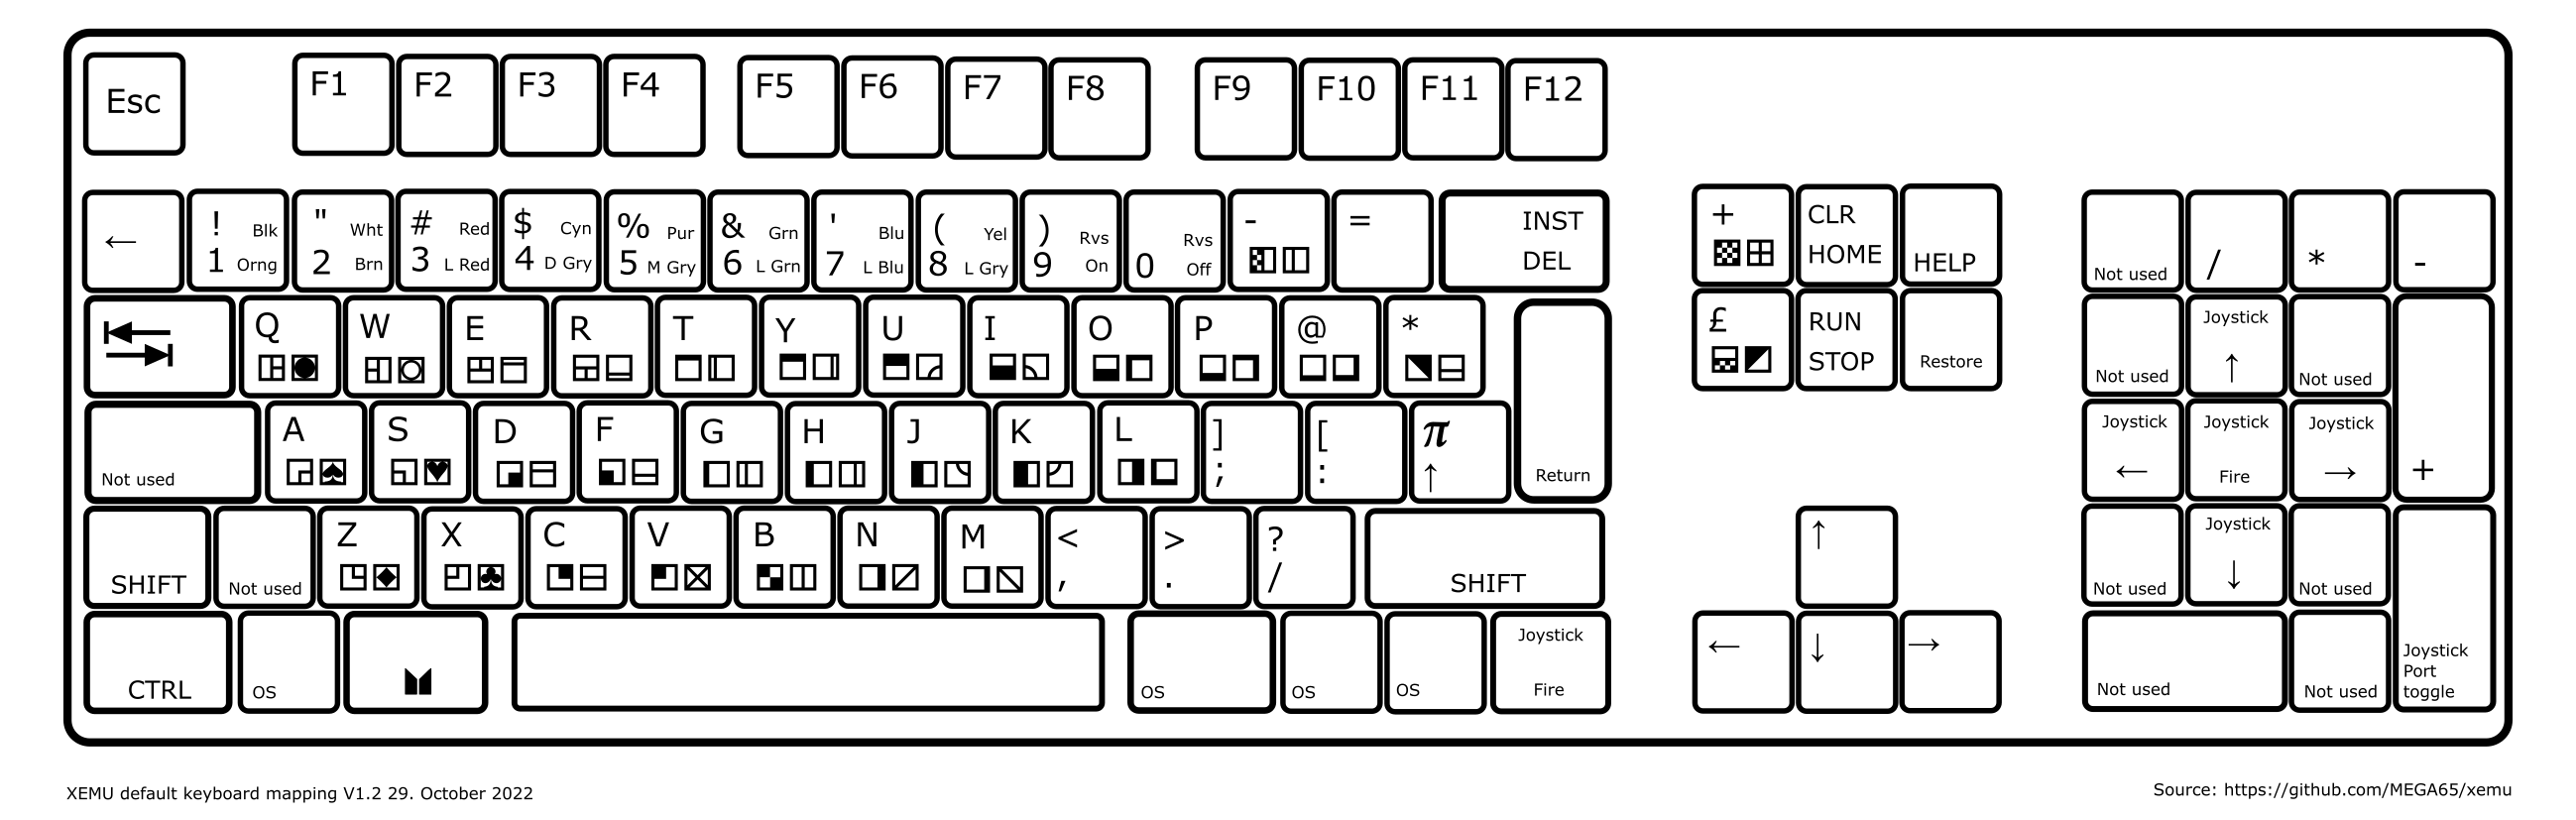
\includegraphics[width=\linewidth]{images/xemu-extended-keyboard.png}
\end{center}

On most PC keyboards, this places \specialkey{RUN STOP} and \widekey{RESTORE} next to each
other, to make that key combination easy to enter.

This diagram shows the PETSCII glyphs as they appear on a MEGA65 keyboard, with the
\megasymbolkey glyph on the left and the \specialkey{Shift} glyph on the right. Note
that on a PC keyboard, the key for \megasymbolkey is to the right of the
\specialkey{Shift}.

Xemu lets you have two joysticks (one at a time) on the numeric keypad.
\specialkey{Enter} over there is used to toggle ports 1, 2 and to off when pressed
repeatedly.

Please be aware the emulator by default catches \megakey{F9} \megakey{F10}
\megakey{F11} as shortcuts of its own functions. If you want those keys to be used by
the emulated Mega 65 you need to setup an own keyboard mapping. The files are found
in the folder for Xemu's settings as explained on page
\pageref{sec:sdcard-settings-location}. This is done by copying
\stw{keymap-default.cfg} into \stw{keymap.cfg} and then removing the following lines:

\begin{tcolorbox}[colback=black,coltext=white]
\verbatimfont{\codefont}
\begin{verbatim}
XEMU-EXIT F9
XEMU-FULLSCREEN F11
\end{verbatim}
\end{tcolorbox}

and changing:

\begin{tcolorbox}[colback=black,coltext=white]
\verbatimfont{\codefont}
\begin{verbatim}
F9 Unknown
F11 Unknown
\end{verbatim}
\end{tcolorbox}

into:

\begin{tcolorbox}[colback=black,coltext=white]
\verbatimfont{\codefont}
\begin{verbatim}
F9 F9
F11 F11
\end{verbatim}
\end{tcolorbox}

Fullscreen and exiting Xemu is still available in the menu you reach by right mouse
clicking into the emu's main window.

\subsection{Apple MacOS start problems}

If a message \stw{macOS cannot verify that this app is free from malware} pops up you
may want control-click to start it: \index{Apple} \index{macOS}

\begin{itemize}
  \item Open Finder on your Mac.
  \item Point your mouse to Xemu's app icon.
  \item Control-click it to open the shortcut menu.
  \item Now click \stw{Open} to run Xemu. By doing it this way no warning will be shown.
\end{itemize}

\subsection{Updating settings}
\label{sec:sdcard-settings-location}
\index{SD card}

You may wish to edit the Xemu settings file to change the keyboard mapping or set the
default SD card image file. To access this file from within Xemu, open the menu,
select \stw{Debug / Advanced} then \stw{Browse system folder}. Edit the
\stw{keymap-default.cfg} and \stw{mega65-default.cfg} files with a text editor.

\begin{center}
  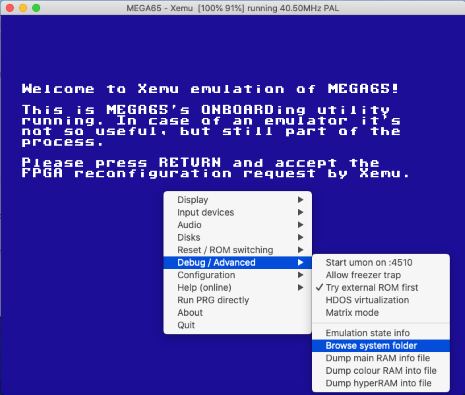
\includegraphics[width=0.5\linewidth]{images/xemusettings.png}
\end{center}

The Xemu system folder location varies by operating system:

\begin{itemize}
    \item Windows:
    \stw{\%appdata\%$\textbackslash$xemu-lgb$\textbackslash$mega65}
    \item Linux:
    \stw{$\textasciitilde$/.xemu-lgb/}
    \item Macintosh:
    \stw{$\textasciitilde$/Library/Application$\textbackslash$ Support/xemu-lgb/mega65/}
\end{itemize}


\section{Using the Live ISO image}
\label{sec:live-iso-image}

The Live ISO image is the product of a volunteer community; not the MEGA65 team. We include it for your convenience.

\subsection{Creating a Bootable USB stick or DVD}

There are many ways to create a live ISO image. The method you choose depends on your operating system and whether you wish to install to a USB drive or burn it to a DVD. Burning to a DVD is straightforward, assuming you own a computer that has a DVD writer. If you wish to create a faster bootable USB drive, try one of the methods below:

If you are using Windows, consider a tool like \url{http://www.isotousb.com/}.

On Linux, you can use the instructions at \url{https://fossbytes.com/create-bootable-usb-media-from-iso-ubuntu/}.

For Apple Macs, consider these instructions at
\url{https://ubuntu.com/tutorials/create-a-usb-stick-on-macos#1-overview}.

Similar instructions are available for other popular computers, such as Amigas (\url{https://forum.hyperion-entertainment.com/viewtopic.php?t=3857}), or Sun UltraSPARC workstations (\url{https://forums.servethehome.com/index.php?threads/how-to-create-a-bootable-solaris-11-usb.1998/}).

Finally, the popular, easy-to-use, and free cross-platform belanaEtcher is available at \url{https://www.balena.io/etcher/}.

\subsection{Getting Started}

To avoid potential copyright issues, the bootable ISO image does not include proprietary ROMs for the MEGA65; such as legacy C65 ROMs. It does include an open-source replacement ROM from our OpenROMs project.\index{OpenROMs} This ROM will boot into a BASIC 2 environment that you can use to load and execute many C64 programs as shown in the image below:

\screenshotwrap{images/liveiso-openrom.png}

If you wish to use a C65 ROM that includes BASIC 10, download the appropriate ROM file and place it on another USB stick named \stw{MEGA65.ROM}. On start-up, the MEGA65 will ask if a ROM has been downloaded; as shown in the image below:

\screenshotwrap{images/liveiso-rom-usb-prompt.png}

If the Live ISO cannot find a ROM, it will prompt you to download a ROM; as shown below:

\screenshotwrap{images/liveiso-rom-download-prompt.png}

\subsection{Other Features of the Live ISO}

As the previous screen-shots show, the Live ISO provides various and convenient desktop shortcuts. On the left-hand side, there are shortcuts for launching the
MEGA65 emulator and the C65 emulator so you can test that programs
will run on both platforms. As previously mentioned, both emulators are a work in progress and may not be 100\% compatiable.

Another link provides access to the MEGA65 Book. This all-in-one volume, of apporixmately 800 pages, contains the official MEGA65 documentation. The majority of this developer's guide is also present in the MEGA65 Book.

This ISO also includes documentation for the C65 Notepad; a program for the C65 and MEGA65 written by Snoopy (the developer of the Live ISO image). A ``read me'' file contains further information about the Live ISO.

Finally, on the right-hand side, there are links to download a C65 ROM and to update the MEGA65 Book to the latest version. This will ensure you don't need to create a new bootable image each time a frequent update is made to the MEGA65 Book.

To access all contents of the Live ISO image, use the file explorer.

% 2021-03-17 edits by SBC
